\documentclass[12pt]{article}

\usepackage{fullpage}
\usepackage{multicol,multirow}
\usepackage{tabularx}
\usepackage{ulem}
\usepackage[utf8]{inputenc}
\usepackage[russian]{babel}
\usepackage{minted}
\usepackage{graphicx}

% Оригиналный шаблон: http://k806.ru/dalabs/da-report-template-2012.tex

\begin{document}
\begin{titlepage}
\begin{center}
\textbf{МИНИСТЕРСТВО ОБРАЗОВАНИЯ И НАУКИ РОССИЙСОЙ ФЕДЕРАЦИИ
\medskip
МОСКОВСКИЙ АВЦИАЦИОННЫЙ ИНСТИТУТ
(НАЦИОНАЛЬНЫЙ ИССЛЕДОВАТЬЕЛЬСКИЙ УНИВЕРСТИТЕТ)
\vfill\vfill
{\Huge ЛАБОРАТОРНАЯ РАБОТА №2}\\
по курсу операционные системы\\
I семестр, 2019/20 уч. год}
\end{center}
\vfill

Студент \uline{\it {Попов Данила Андреевич, группа 08-208Б-18}\hfill}

Преподаватель \uline{\it {Миронов Евгений Сергеевич}\hfill}

\vfill
\end{titlepage}

\subsection*{Условие}

Написать программу, которая рекурсивно вычисляет n-ое число Фибоначи.

\subsection*{Описание программы}

Код программы состоит из 3-х файлов:
\begin{enumerate}
\item main.c: файл, содержащий точку входа приложения и верхний уровень абстракции реализации рекурсии.
\item childprocess.h: файл, содержащий объявление функций, необходимых для создания дочерних процессов.
\item childprocess.c: файл, содержащий реализацию функций, необходимых для создания дочерних процессов.
\end{enumerate}

\subsection*{Ход выполнения программы}
\begin{enumerate}
\item Чтение индекса n вычисляемого числа Фибоначи.
\item Если индекс достаточно велик, то создаётся два дочерних процесса с перенаправленными потоками ввода и вывода:
\begin{enumerate}
\item Передача в дочерние процессы через перенаправленные потоки ввода n - 1 и n - 2 соответственно.
\item Чтение результатов через перенаправленные потоки вывода дочерних процессов.
\item Суммирование результатов.
\end{enumerate}
Иначе выбирается заранее вычисленное число по индексу.
\item Вывод конечного результата в стандартный поток вывода.
\item Завершение работы программы.
\end{enumerate}

\subsection*{Недочёты}
Примерно 65000 активных процессов при вычислении 16-го числа.

\subsection*{Выводы}
Рекурсивное вычисление чисел Фибоначи через создание дочерних процессов --- не лучший способ решения данной задачи.
\pagebreak

\subsection*{Вывод программы}
4\\
2

\subsection*{procmon log}
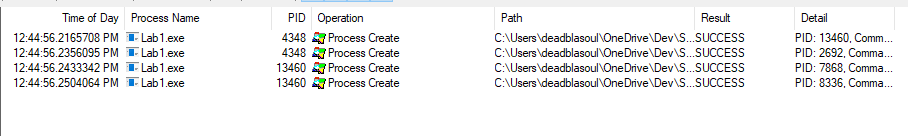
\includegraphics[scale=0.65]{report.png}

\pagebreak

\subsection*{Исходный код}

{\Huge main.c}
\inputminted
{C++}{main.c}
\pagebreak

{\Huge childprocess.h}
\inputminted
{C++}{childprocess.h}
\pagebreak

{\Huge childprocess.c}
\inputminted
{C++}{childprocess.c}
\pagebreak

\end{document}
